\documentclass{article}
\usepackage{amsmath}
\usepackage{pgfplots}
\usepackage{enumitem}
\author{Tianyu Du}
\date{Since Sep 2017}
\title{Notes on PSY100}
\begin{document}
	\maketitle
	\tableofcontents
	\section{Welcoming Sep7}
	\paragraph{}The purpose of psychology is to give us a \textbf{completely different} idea of the \textbf{things we know best}. \emph{Attributed to French poet Paul Valery}
	\paragraph{Experimental Psychology} \emph{Wilhelm Wundt} \emph{Leipzig, Germany}
	\paragraph{New Items}
	\begin{itemize}
		\item Structuralism \newline Descriptive.
		\item Functionalism \newline Understand how consciousness works, inspired by \textbf{Evolutionary Theory}.
		\item Behaviourism \newline Mind is a \textbf{Black Box}, focus stimulus and responses.
		\item Humanism \newline Psychical analysis. Personality.
	\end{itemize}
	\paragraph{Course structures}
	\begin{enumerate}
		\item Research Methods.
		\item \begin{enumerate}
			\item Biological.
			\item Developmental.
			\item Cognitive.
			\item Social \& personalty.
			\item Mental psychical health.
		\end{enumerate}
		\item Integration.
	\end{enumerate}
	\section{Sep14 2017}
	\paragraph{Variables} A characteristic or condition that changes or has different values for different individuals.
	\begin{itemize}
		\item \textbf{Independent variable} A variable that is \emph{manipulated}, in order to see its impact on the dependent variable.
		\item \textbf{Dependent variable} A variable that is \emph{measured} in order to see how it is affected by the independent variable.
		\item \textbf{Operational definitions} Definitions of theoretical constructs that are sated in term of concrete, observable procedures.
			\newline \textbf{Construct} Internal attributes or characteristics that cannot be directly observed but are useful for describing and explaining behaviour.
			\begin{itemize}
				\item Physiological measure.
				\item Behavioural measure.
				\item Self-reported measure.
			\end{itemize}
	\end{itemize}
	\paragraph{Types of Research \& Subsequent Claims}
	\begin{itemize}
		\item \textbf{Descriptive Research}
		\begin{itemize}
			\item Observations, case studies.
			\item May result in claims regarding the \emph{frequency of some behaviour}.
		\end{itemize}
		\item \textbf{Correlational Research}
		\begin{itemize}
			\item May lead to claims regrading to the \emph{association between variables}.
		\end{itemize}
		\item \textbf{Experimental Research}
		\begin{itemize}
			\item May lead to claims regarding to the \emph{casual relationship} between two variables.
		\end{itemize}
	\end{itemize}
	\paragraph{Confound}: Anything that may unintentionally vary along with the independent variable.
	\paragraph{Random assignment} Each participant has an equal chance being assigned to each experimental condition.
	\newline \emph{Necessary Component} of experiment.
	\paragraph{Random sample} Each member of the population you are interested in has an equal change of being chosen to participate.
	\section{Sep. 21 The Nervous System}
	\begin{itemize}
		\item Central nervous system (CNS)
		\begin{itemize}
			\item Brain \& Spinal cord.
		\end{itemize}
		\item Peripheral nervous system (PNS)
		\begin{itemize}
			\item Somatic nervous system.
			\item Autonomic nervous system.
		\end{itemize}
	\end{itemize}
	\section{Notes on slides: Biological Foundations of Behaviour, Sep. 19. 2017}
	\paragraph{Twin Studies \& Adoption Studies}
	\begin{itemize}
		\item Compare impact of \textbf{genetic} and \textbf{environmental} influences.
		\item \textbf{Monozygotic} and \textbf{dizygotic}.
	\end{itemize}
	\paragraph{Epigenetic} \emph{Epi $\rightarrow$ Outer} Changes in gene expression that are due to non-genetic influences.
	\subsection{Heredity v.s. Heritability}
	\paragraph{Heredity} Genetic transmission of characteristics from parents to offspring.
	\paragraph{Heritability(Coefficient)} An estimate of the \emph{genetic proportion} of the variation in some specific trait.
	\begin{itemize}
		\item Within \textbf{population} (not individual).
		\item \textbf{\%} of \textbf{variation} explained by genetic differences.
	\end{itemize}
	\subsection{The Nervous System}
	\paragraph{Central Nervous System(CNS)}
	\begin{itemize}
		\item \textbf{Brain}.
		\item \textbf{Spinal cord}.
	\end{itemize}
	\paragraph{Peripheral Nervous System(PNS)}
	\begin{itemize}
		\item \textbf{Somatic nervous system}.
		\item \textbf{Autonomic nervous system}.
		\begin{itemize}
			\item Sympathetic nervous system.
			\item Parasympathetic nervous system.
		\end{itemize}
	\end{itemize}
	\subsection{Neurons}
	\begin{itemize}
		\item \textbf{Sensory} $\rightarrow$ Afferent.
		\item \textbf{Motor neurons} $\rightarrow$ Efferent.
		\item Interneurons.
	\end{itemize}
	\begin{figure}
		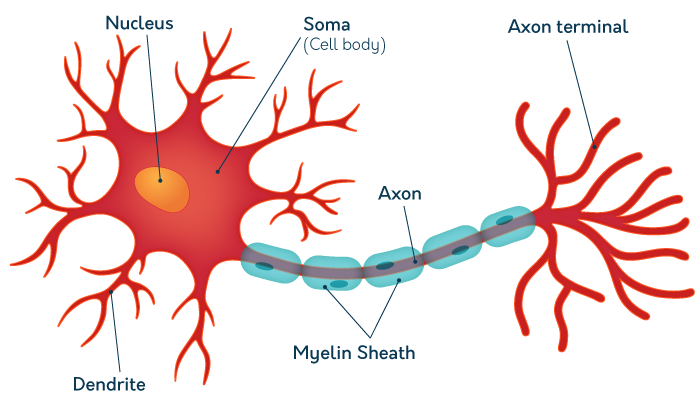
\includegraphics[width=\linewidth]{/Users/tianyudu/Documents/UToronto/Notes/pic/structure_of_neuron.png}
		\caption{Structure of neuron}
	\end{figure}
	\paragraph{Signals affecting Polarization of the cell.}
	\begin{itemize}
		\item \textbf{Excitatory signals} increase the probability of \emph{firing}.
		\item \textbf{Inhibitory signals} decrease the probability of \emph{firing}.
	\end{itemize}
	\subsubsection{Firing}
	\paragraph{Firing} generates an \textbf{action potential} if excitatory input is larger that \emph{threshold}.
	\paragraph{All or none principle} Neurons fire with \textbf{same} \emph{potency}, with, perhaps, \textbf{different} \emph{frequency}.
	\paragraph{Action potential} the \textbf{neural impulse} that passes along the \textbf{axon} and subsequently causes the release of \textbf{chemical} from the \textbf{terminal buttons}. Action potential originates at the \emph{base} of the axon and rapidly travels down.
	\paragraph{Grey matters}: Cell bodies and dendrites.
	\paragraph{White matters}: Myelinated axons.
	\paragraph{Process of firing:}
	\begin{enumerate}
		\item \textbf{Resting state} Neurons are \emph{polarized} at rest $~= -70 mV$.
		\item \textbf{Depolarization}(if and only if voltage reaches the \emph{threshold}, and the axon will be \emph{fully} depolarized).
		\begin{itemize}
			\item $Na^+$ channels \emph{open}, large amount of $Na^+$ ions get in.
			\item Small amount of $K^+$ ions get out.	
		\end{itemize}
		\item \textbf{Re-polarization}
		\begin{itemize}
			\item $Na^+$ channels \emph{closed}.
			\item $K^+$ channels \emph{open}, large amount of $K^+$ ions get out.
		\end{itemize}
		\item \textbf{Hyper-polarization} (\emph{over-shooting}), during this \textbf{refractory} period, neuron can \textbf{not} fire.
		\item \textbf{Rest state} $k^+$ channels \emph{closed}, voltage increases back to \emph{rest state}. 
	\end{enumerate}
	\begin{figure}
		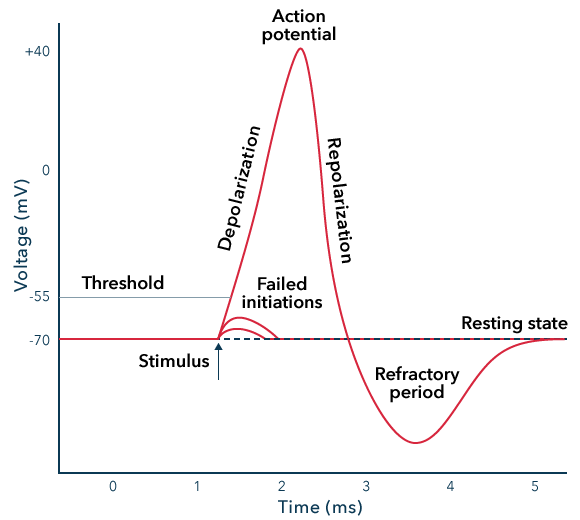
\includegraphics[width=\linewidth]{pic/voltage.png}
		\caption{Voltage changes in axon when neurons is firing.}	
	\end{figure}

	\subsection{Neurotransmitter}
	\paragraph{Neurotransmitter} is \emph{chemical} substances carry \emph{signals} between neurons. And neurotransmitters are stored in \textbf{vesicles}.
	\begin{figure}
		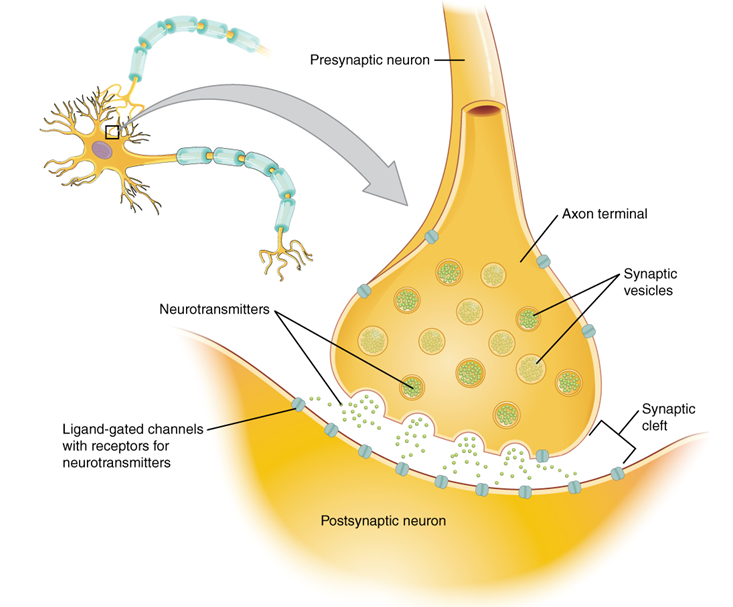
\includegraphics[width=\linewidth]{pic/transmitter}
		\caption{Neurotransmitters, vesicles, terminal buttons and dendrites.}
	\end{figure}
	\begin{table}
		\centering
		\begin{tabular}{|c|c|}
			\hline
			\textbf{Neurotransmitter} & \textbf{Usages} \\ \hline
			Glutamate & Primary \textbf{excitatory} transmitter.\\ \hline
			GABA & Primary \textbf{inhibitory} transmitter.\\ \hline
			Serotonin & Mood, impulsiveness, hunger and sleep.\\ \hline
			Dopamine & Reward and motivation, voluntary movement.\\ \hline
			Acetylcholine & Motor control (nerves and muscles), memory, sleep. \\ \hline
			Epinephrine(Adrenaline) & energy \\ \hline
			Norepinephrine & Arousal, alterness \\ \hline
		\end{tabular}
		\caption{Common neurotransmitters}
	\end{table}
	\subsubsection{Drugs}
	\paragraph{Agonists} \textbf{Enhance} neurotransmitters' actions.
	\begin{itemize}
		\item \textbf{Increase} the \textbf{release} of neurotransmitter.
		\item \textbf{Block} the \textbf{pre-take up} neurotransmitter.
		\item \textbf{Mimicking} a neurotransmitter to activate a postsynaptic receptor.
	\end{itemize}
	\paragraph{Antagonists} \textbf{Inhibit} neurotransmitters' actions.
	\begin{itemize}
		\item \textbf{Block} the \textbf{release} of neurotransmitter.
		\item \textbf{Destroy} neurotransmitter in the synapse.
		\item \textbf{Mimicking} a neurotransmitter.
	\end{itemize}
	\subsection{Brains: From the button up}
	\paragraph{Contralateral control} Nervous carrying motor and sensory information \emph{crossover}.
	\newline Right somatosensory cortex process left side of body.
	\begin{itemize}
		\item \textbf{Cerebral cortex}: complex \emph{mental} activities.
		\item \textbf{Limbic system}: emotions and basic drives.
		\item \textbf{Basal ganglia \& cerebellum}: movement.
		\item \textbf{Brainstem}: Survival.
	\end{itemize}
	\subsubsection{brainstem}
	\begin{enumerate}
		\item Med brain.
		\item Pons.
		\item Medulla.
	\end{enumerate}
	\paragraph{Function:}Reticular formation(alertness and sleeping).
	\subsubsection{Cerebellum}
	\paragraph{Function:}Coordinate \textbf{movement} and \textbf{balance}.
	\subsubsection{Hypo-thalamus}
	\paragraph{Function:} Master \textbf{regulatory structure} and link \emph{nervous system} and \emph{endocrine system}.
	\subsubsection{Thalamus}
	\paragraph{}\textbf{Gateway} to the brain.
	\paragraph{}Handles all incoming sensory information \textbf{except smell}.
	\subsubsection{Hippocampus}
	\paragraph{}Memories.
	\subsubsection{Amygdala}
	\paragraph{} Emotional and \emph{intensifies} memory when \textbf{emotional arousal}.
	\subsubsection{Cingulate gyrus.}
	\paragraph{} Regulating \textbf{emotions} and \textbf{pain}(both \emph{physical} and \emph{social} pain). \emph{Predicting and avoiding}.
	\subsubsection{Basal ganglia}
	\paragraph{Subcortical nuclei}
	\begin{enumerate}[label=\roman*).]
		\item Caudata nucleus.
		\item Putamen.
		\item Globus pallidus
		\item Nucleus accumbens. 
	\end{enumerate}
	\paragraph{Producing/Planning movement}\[
	\text{\textbf{Cortex}} \rightarrow \text{\textbf{Basal ganglia}} \rightarrow \text{\textbf{Motor centers of brainstem}}
	\]
	\subsubsection{Cerebral cortex}
	\begin{figure}
		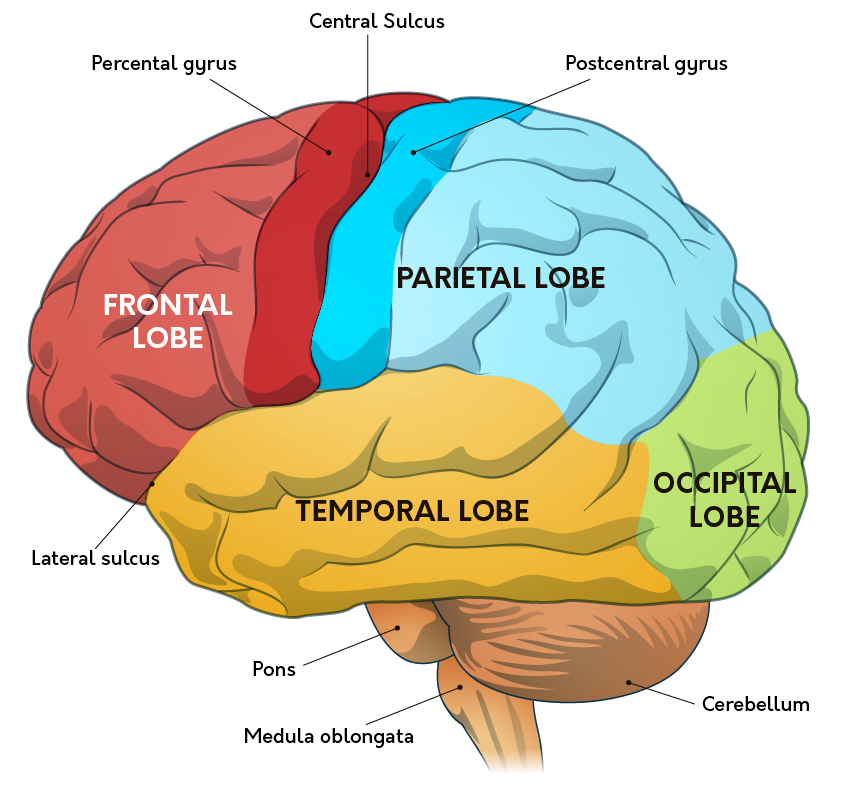
\includegraphics[width=\linewidth]{pic/brain_structure.png}
		\caption{Structure of brain.}
	\end{figure}
	\begin{figure}
		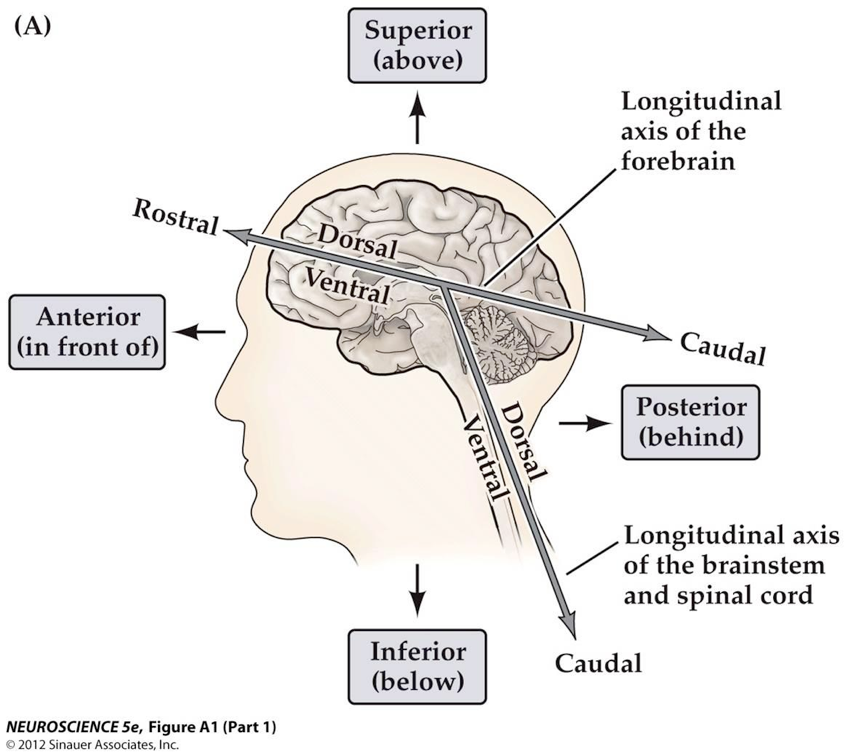
\includegraphics[width=\linewidth]{pic/brain_pos.png}
		\caption{Structure of brain.}
	\end{figure}
	\subsection{Four Lobes in each hemisphere}
	\subsubsection{Frontal lobe}
		\begin{itemize}
			\item Primary \textbf{motor} cortex.
			\item \textbf{Prefrontal cortex}.
		\end{itemize}
	\subsubsection{Pariental lobe}
		\begin{itemize}
			\item Primary \textbf{somatosensory} (\emph{touch}) cortex.
		\end{itemize}
	\subsubsection{Temporal lobe}
		\begin{itemize}
			\item Primary \textbf{auditory} cortex.
		\end{itemize}
	\subsubsection{Occipital lobe}
		\begin{itemize}
			\item Primary \textbf{visual} cortex.
		\end{itemize}
	\paragraph{Prefrontal cortex:} 30\% of human brain.
	\paragraph{Cortical sensory} representing each part of body. Connected parts of the body tend. to be represented beside each other. Sensitive regions trend to have larger cortical area.
	\paragraph{Plasticity} The ability to \emph{change}, \emph{reorganize}, as a result of \emph{experience}, \emph{drugs}, \emph{injury}.
	\subsection{The peripheral nervous system}
	\paragraph{Functions:}
	\begin{enumerate}[label=\roman*).]
		\item Trans. information to central nervous system.
		\item Responds to information from central nervous system.
	\end{enumerate}

	\paragraph{Contents:}
	\begin{enumerate}[label=\roman*).]
		\item Somatic nervous system (SNS).
			\begin{enumerate}[label=\alph*).]
				\item Concern \textbf{external} environment.
				\item Conscious/voluntary control.
				\item Motor nervous (signals from the brain to the muscles).
				\item Sensory neurons.
			\end{enumerate}
		\item Autonomic nervous system (ANS).
			\begin{enumerate}[label=\alph*).]
				\item Concern \textbf{internal} environment.
				\item Divisions of the ANS.
				\begin{itemize}
					\item \textbf{Sympathetic}: prepare body for actions.
						\newline $\updownarrow$ \emph{complementary} $\updownarrow$	
					\item \textbf{Parasympathetic}: return body to normal state.
				\end{itemize}
			\end{enumerate}	
	\end{enumerate}
	\subsection{Endocrine system}
	\paragraph{Function:} Regulate psychological activities with nervous system.
	\paragraph{Difference between endocrine system and nervous system}
	\begin{itemize}
		\item \textbf{Endocrine system}: Release \textbf{Hormones}(\emph{chemicals} from \textbf{endocrine glands}) into blood stream. So the effects are \emph{slower} but \emph{long lasting} and \emph{widespread}.
		\item \textbf{Nervous system}: Release \textbf{electrochemical} signals.
	\end{itemize}
	\subsection{Coordinated system}
	\paragraph{} Hypothalamus connects the systems and control \textbf{pituitary gland}.
	\paragraph{Process:}
	\begin{enumerate}
		\item \textbf{Neural activation}
		\item \textbf{Hypothalamus} secrete releasing factors.
		\item \textbf{Pituitary gland} releases hormones.
		\item \textbf{Hormones} travel through blood stream to the target.
	\end{enumerate}
\end{document}





















